
\section{Entropy stability}
\label{sec:EV-ME}

Earlier in the thesis (\cref{sec:Background:C-ES-scalar-LTS,sec:LTS-HLL:C-ES-scalar-LTS}), we have seen that the tools commonly used to prove entropy stability of standard methods are not readily available for LTS methods. Therein, we postponed the discussion on entropy stability in LTS methods, and now we finally address it by using modified equation. We begin this section with a word of caution:
\begin{quote}
\small
\textit{"Modified equations have been a commonly used tool in the study of difference schemes. Because of the lack of any theoretical foundation, this use has been accompanied by constant difficulties and results derived from modified equations have sometimes been
regarded with apprehension. As a result, a situation arises where authors either
disregard entirely the technique or have an unjustified faith in its scope."}
\qauthor{Griffiths and Sanz-Serna~\cite{gri86}}
\end{quote}
\vspace{-2.5mm}
We are hoping to avoid both of these pitfalls, and to use modified equation while being fully aware that it is based on certain assumptions that prevent us from using it as a tool to rigorously prove entropy stability. With this in mind we proceed to use modified equation analysis to conjecture about the entropy stability of the LTS-HLL-type schemes.

We start by outlining how entropy violation happens in standard methods following the \textit{numerical viscosity} interpretation~\cite{lev02}. We then move to LTS methods, and present new difficulties that arise in LTS framework and different ways how this is handled in the existing literature. By following the modified equation analysis by Lindqvist et al.~\cite{lin16}, we illustrate the mechanism behind the entropy violation in the LTS-Roe scheme. Then, we show how is it avoided in some LTS-HLL-type schemes.

Part of discussion in this section closely follows our conference paper~\cite{cp2}. The major difference is that here we focus on scalar conservation laws, while in the paper we consider the Euler equations.

\subsection{Entropy violation}

Entropy violation is most commonly associated and discussed as it appears in the Roe scheme~\cite{roe81}. Therefore, we focus on the Roe scheme and start by following the numerical viscosity interpretation of the entropy violation as found in the book by LeVeque~\cite{lev02}.

The numerical flux function of the Roe scheme can be written as:
\begin{equation}
F_{j+1/2}^\text{Roe} = \frac{1}{2} \left( f_j + f_{j+1} \right) - \frac{1}{2} \left| \lambda_{j+1/2} \right| \left( u_{j+1} - u_j \right),
\end{equation}
where we recall that $ \lambda_{j+1/2} $ was defined in \eqref{eq:scalar-lambda}. In the case of a transonic rarefaction, $ f'(u_j) < 0 < f'(u_{j+1}) $, the shock speed may be very close to zero, corresponding to no viscosity. We define the interface Courant number $ C_{j+1/2} = \lambda_{j+1/2} \Delta t / \Delta x $ and note that if:
\begin{equation} \label{eq:scalar-standard-EV}
C_{j+1/2} = 0,
\end{equation}
we might obtain an entropy violation, because in case of a transonic rarefaction the exact solution is supposed to be a rarefaction wave \eqref{eq:scalar-rarefaction}, while the Roe scheme will treat it as a stationary shock with the velocity $ \lambda_{j+1/2}=0 $. For the standard methods, these situations are well understood and we refer to~\cite{lev02} and references therein for more detailed discussions.

For the LTS-Roe scheme, most of authors observed that it leads to entropy violations more often than the standard Roe scheme~\cite{lev82,lev85,qia11,mor12a,xu14,lin16,lin16b}. Lindqvist et al.~\cite{lin16} showed that such LTS-related entropy violation may appear when:
\begin{equation} \label{eq:scalar-LTS-EV}
C_{j+1/2} = -i, \quad \forall \, i \, \in \, \mathbb{Z}.
\end{equation}
In earlier papers on LTS methods, this issue is solved by manually splitting the rarefaction wave into several expansion shocks~\cite{lev82,lev85,qia11,mor12a,xu14} or by varying the time step~\cite{lin16b,lin16}. We now show how this issue is automatically avoided in the LTS-HLLE and LTS-Rusanov schemes.

\subsection{Modified equation analysis}

For the standard one-parameter method we may gain insight into the numerical viscosity of the method by looking at the numerical flux function and the corresponding numerical viscosity coefficient $ Q $. However, for LTS methods the numerical flux function contains multiple numerical viscosity coefficients, so it is more convenient to work with the modified equation.

Earlier on (\cref{sec:Background:C-ES-scalar-LTS,sec:LTS-HLL:C-ES-scalar-LTS}) we have seen that a first-order LTS methods give a second-order accurate approximation to the equation:
\begin{equation} \label{eq:LTS-ME4}
u_t + f(u)_x = \frac{1}{2} \frac{\Delta x^2}{\Delta t} \left[ D u_x \right]_x,
\end{equation}
where the inherent numerical diffusion was already introduced for standard schemes \eqref{eq:ME-D}:
\begin{equation} \label{eq:LTS-ME-D}
D = \sum\limits_{i=1-k}^{k-1} \frac{\Delta t}{\Delta x} \bar{Q}^i - c^2.
\end{equation}
Lindqvist et al.~\cite{lin16} determined the inherent numerical diffusion of the LTS-Roe and LTS-Lax-Friedrichs schemes:
\begin{align}
D_\text{LTS-Roe} & = \left( \lceil |c| \rceil - |c| \right) \left( 1 + |c| - \lceil |c| \rceil \right), \label{eq:D-LTS-Roe} \\
D_\text{LTS-LxF} & = k^2 - c^2. \label{eq:D-LTS-LxF}
\end{align}
In our conference paper~\cite{cp2} we determined it for the LTS-HLL scheme:
\begin{align} \label{eq:D-LTS-HLL}
D_\text{LTS-HLL} & = \frac{c - \CL}{\CR - \CL} \left( \lceil |\CR| \rceil - |\CR| \right) \left( 1 + |\CR| - \lceil |\CR| \rceil \right) \notag \\ 
& + \frac{\CR - c}{\CR - \CL} \left( \lceil |\CL| \rceil - |\CL| \right) \left( 1 + |\CL| - \lceil |\CL| \rceil \right) \notag \\ 
& + \left( c - \CL \right) \left( \CR - c \right),
\end{align}
where we recall that we defined $ \CL = \SL \Delta t / \Delta x $, $ \CR = \SR \Delta t / \Delta x $ and \mbox{$ c = f'(u) \Delta t / \Delta x $}, where $ \lceil c \rceil = \min \{ n \in \mathbb{Z} \,| \, n \geq c \} $ is the ceiling function.

We can observe that the inherent numerical diffusion of the LTS-Roe scheme \eqref{eq:D-LTS-Roe} vanishes when the condition \eqref{eq:scalar-LTS-EV} is satisfied, leading to no diffusion being introduced by the method. If the exact solution is a rarefaction wave, this will lead to an entropy violation. This does not happen in the LTS-HLLE scheme:
\begin{proposition}[Prebeg~\cite{cp2}] \label{prop:LTS-HLL-D}
If the exact solution of the Riemann problem is a rarefaction wave, i.e.:
\begin{equation} \label{eq:scalar-LaxEC}
f'(u_j) < \lambda_{j+1/2} < f'(u_{j+1}),
\end{equation}
the inherent numerical diffusion of the LTS-HLLE scheme satisfies:
\begin{equation}
D_\textup{LTS-HLLE} > 0.
\end{equation}
\end{proposition}
\begin{proof}
In the HLLE scheme, the wave velocity estimates are:
\begin{subequations} \label{eq:scalar-Einfeldt2}
\begin{align}
\SL & = \min \left( \lambda_{j+1/2}, f'(u_j) \right), \\
\SR & = \max \left( \lambda_{j+1/2}, f'(u_{j+1}) \right).
\end{align}
\end{subequations}
If \eqref{eq:scalar-LaxEC} holds, then \eqref{eq:scalar-Einfeldt2} yields:
\begin{equation}
\SL = f'(u_j) < \lambda_{j+1/2} < \SR = f'(u_{j+1}).
\end{equation}
By using these in \eqref{eq:D-LTS-HLL} we observe that:
\begin{equation}
D_\textup{LTS-HLLE} \geq \left( c - \CL \right) \left( \CR - c \right) > 0. 
\end{equation}
\end{proof}
We can see that if the solution to the Riemann problem is a rarefaction wave, the LTS-HLLE scheme always introduces a certain amount of numerical diffusion. This is due to the fact that the HLLE scheme splits each discontinuity into two waves, and it is in fact entropy stable. We recall that LeVeque conjectured that the LTS-Godunov method converges to the unique entropy solution if we use the entropy solution for each Riemann problem~\cite{lev84} (see also page~\pageref{sec:LTS-entropy-stability} of this thesis). This conjecture holds for any Riemann solver that itself satisfies the entropy condition, so we conjecture that the LTS-HLLE scheme converges to the entropy solution, because we use the entropy stable solution for each Riemann problem. 

\subsection{A class of one-parameter modified equations}

Following the reasoning we used to deduce standard one-parameter methods from the HLL-type scheme~(\Cref{prop:HLL-NV-Qs,prop:HLL-FDS-As}), and to deduce LTS one-parameter methods from the LTS-HLL-type scheme~(\Cref{prop:LTS-HLL-NV-Qs,prop:LTS-HLL-FDS-As}), we establish the equivalent result for the modified equations.

\begin{proposition}
A first-order accurate, LTS one-parameter conservative scheme written in the numerical viscosity form \eqref{eq:scalar-LTS-NV}, which is uniquely determined by the partial numerical viscosity coefficients $ Q_\text{S}^i $, gives a second-order accurate approximation to the equation:
\begin{equation} 
u_t + f(u)_x = \frac{1}{2} \frac{\Delta x^2}{\Delta t} \left[ D_\text{S} u_x \right]_x,
\end{equation}
where the inherent numerical diffusion is:
\begin{equation} \label{eq:LTS-ME-oneQ}
D_\text{S} = c_\text{S} \left( 2 \lceil c_\text{S} \rceil - 1 \right) + \lceil c_\text{S} \rceil \left( 1 - \lceil c_\text{S} \rceil \right) - c^2,
\end{equation}
with $ c_\text{S} = Q_\text{S} \Delta t / \Delta x $.
\end{proposition}

\begin{proof}
The derivation of the modified equation for the LTS-HLL-type scheme \eqref{eq:D-LTS-HLL} makes no assumptions on the choice of $ \SL $ and $ \SR $. Hence, we may define $ \SL=-Q_\text{S} $ and $ \SR=Q_\text{S} $ in \eqref{eq:D-LTS-HLL}, which then reduces to \eqref{eq:LTS-ME-oneQ}.
\end{proof}

For $ c_\text{S} = c $ and for $ c_\text{S} = k $, this reduces to the modified equations of the LTS-Roe \eqref{eq:D-LTS-Roe} and LTS-Lax-Friedrichs schemes \eqref{eq:D-LTS-LxF}, respectively.
Following \Cref{prop:LTS-HLL-D}, we can show the same result for the LTS-Rusanov scheme.

\begin{proposition} \label{prop:LTS-Rus-D}
If the exact solution of the Riemann problem is a rarefaction wave, i.e.:
\begin{equation} \label{eq:scalar-LaxEC2}
f'(u_j) < \lambda_{j+1/2} < f'(u_{j+1}),
\end{equation}
the inherent numerical diffusion of the LTS-Rusanov scheme satisfies:
\begin{equation}
D_\textup{LTS-Rus} > 0.
\end{equation}
\end{proposition}
\begin{proof}
With the Rusanov scheme, the numerical viscosity coefficient is:
\begin{equation} \label{eq:scalar-Rusanov-Q}
Q_\text{Rus} = \max \left( |\lambda_j|, |\lambda_{j+1}| \right) = \max \left( |f'(u_j)|, |f'(u_{j+1})| \right).
\end{equation}
If \eqref{eq:scalar-LaxEC2} holds, then using \eqref{eq:scalar-Rusanov-Q} in \eqref{eq:LTS-ME-oneQ} and rewriting yields:
\begin{equation}
D_\textup{LTS-Rus} = \left( \lceil |c_\text{Rus}| \rceil - |c_\text{Rus}| \right) \left( 1 + |c_\text{Rus}| - \lceil |c_\text{Rus}| \rceil \right) + c_\text{Rus}^2 - c^2,
\end{equation}
where $ c_\text{Rus} = Q_\text{Rus} \Delta t / \Delta x $. The first term has the same form as the LTS-Roe scheme \eqref{eq:D-LTS-Roe}:
\begin{equation}
\left( \lceil |c_\text{Rus}| \rceil - |c_\text{Rus}| \right) \left( 1 + |c_\text{Rus}| - \lceil |c_\text{Rus}| \rceil \right) \geq 0,
\end{equation}
and since $ c_\text{Rus} > c $, the second term is:
\begin{equation}
c_\text{Rus}^2 - c^2 > 0.
\end{equation}
Hence we have that:
\begin{equation}
D_\textup{LTS-Rus} > 0.
\end{equation}
\end{proof}
We may also make certain observations about our LTS extensions of other one-parameter methods mentioned on page~\pageref{eq:LTS-1p-itemize}:
\begin{itemize}
\item \textit{LTS-Godunov:} NV coefficient of the standard Godunov scheme differs from the NV coefficient of the standard Roe scheme only in the case of a transonic rarefaction. This property also holds for the LTS-Godunov scheme introduced in this thesis and the LTS-Roe scheme. This means that the LTS-Godunov scheme successfully resolves the transonic rarefaction, but it fails in the same manner as the Roe scheme when the condition \eqref{eq:scalar-LTS-EV} holds.
\item \textit{LTS-Engquist-Osher:} The argument applied for the LTS-Godunov scheme also applies for the LTS-Engquist-Osher scheme.
\item \textit{LTS-Lax-Wendroff:} By choosing $ c_\text{S} = c^2 $, \eqref{eq:LTS-ME-oneQ} yields:
\begin{equation}
D_\text{LTS-L-W} = 2 c^2 \lceil c^2 \rceil - 2c^2 + \lceil c^2 \rceil - \lceil c^2 \rceil^2,
\end{equation}
which vanished only for $ c \leq 1 $. Hence, our LTS-Lax-Wendroff scheme is not second-order accurate.
\end{itemize}

We summarize our observations regarding the entropy stability of LTS methods in the \Cref{tabl:EntropyStability}.

\begin{table}[h!]
\centering

\captionsetup{width=0.65\textwidth}
\caption[whatever]{Entropy stability of different methods: standard and LTS (conjectured\footnotemark)}
\begin{tabular}{@{} c c c c c c c @{}}
\toprule
& Roe & LxF & Rus & E-O & God & HLLE
\\\midrule
Standard  & no & yes & yes & yes & yes & yes \\ 
LTS       & no & yes & yes & no  & no  & yes \\ 
\bottomrule
%\hline
\end{tabular}

\label{tabl:EntropyStability}
\end{table}

\footnotetext{The LTS-Lax-Friedrichs scheme is proved to be entropy stable by proving it is monotone. This will be shown in next section.}

We consider the inviscid Burgers' equation and two Riemann problems:
\noindent\begin{minipage}{\linewidth}
\begin{subequations}
\begin{align} \label{eq:RP-R1}
u(x,0) = \left\{ \begin{array}{ll}
         0 \quad & \text{if} \quad x < 0, \\
         1	     & \text{if} \quad x > 0. \end{array} \right.
\end{align}
\begin{align} \label{eq:RP-R2}
u(x,0) = \left\{ \begin{array}{ll}
         -1 \quad & \text{if} \quad x < 0, \\
         2	      & \text{if} \quad x > 0. \end{array} \right.
\end{align}
\end{subequations}
\phantom \\
\end{minipage}

\Cref{fig:R1} shows the numerical solution to the Riemann problem \eqref{eq:RP-R1} with different LTS methods with $ \bar{C}=5 $ on two different grids on the interval $ x \in [-1,1.5] $. In \Cref{fig:EV-R1-nj100} we see that the LTS-Lax-Friedrichs, LTS-Rusanov and LTS-HLLE successfully resolve the rarefaction, while the LTS-Roe, LTS-Engquist-Osher and LTS-Godunov all lead to the same pattern of entropy violation. This is expected, because for the initial data \eqref{eq:RP-R1} these three schemes are identical. In \Cref{fig:EV-R1-nj100}, the LTS-Lax-Friedrichs scheme leads to a step-like pattern solution, but this is not an entropy violation but a consequence of the fact that the LTS-Lax-Friedrichs scheme splits the discontinuity into two waves, while we only did 8 time steps. \Cref{fig:EV-R1-j1000} shows that as we refine the grid, the LTS-Lax-Friedrichs scheme converges to the exact solution.
\begin{figure}[h!]
	\centering	

	\subfloat[100 cells, $ \Delta t = 0.125 $, 8 time steps]
	{\label{fig:EV-R1-nj100}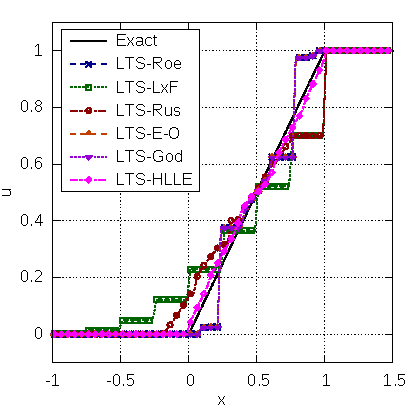
\includegraphics[width=0.48\textwidth]
	{Figures/Scalar/EV-R1-nj100.pdf}}	
	\hspace{0.005\textwidth}
	\subfloat[1000 cells, $ \Delta t = 0.0125 $, 80 time steps]
	{\label{fig:EV-R1-j1000}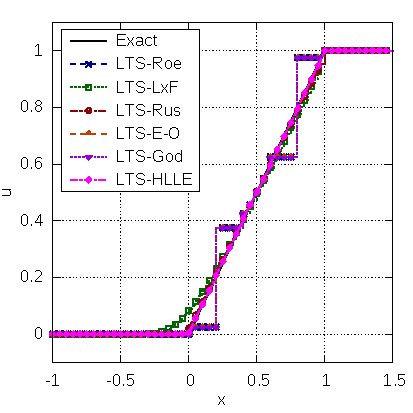
\includegraphics[width=0.48\textwidth]
	{Figures/Scalar/EV-R1-nj1000.pdf}}
	
	\captionsetup{justification=centering}
	
	\caption{Comparison of different LTS methods at $ \bar{C}=5 $ for the Riemann problem \eqref{eq:RP-R1}}
	\label{fig:R1}

\end{figure} 

We now consider a transonic rarefaction. \Cref{fig:R2} shows the numerical solution to the Riemann problem \eqref{eq:RP-R2} with different LTS methods with $ \bar{C}=5 $ on two different grids on the interval $ x \in [-2.5,2.5] $. In \Cref{fig:EV-R2-nj100} we see that the LTS-Lax-Friedrichs, LTS-Rusanov and LTS-HLLE successfully resolve the rarefaction. The LTS-Roe, LTS-Engquist-Osher and LTS-Godunov schemes lead to an entropy violation, but this time in a different manner. The entropy violation in LTS-Roe scheme is a combination of two types of entropy violations -- the standard Roe scheme entropy violation \eqref{eq:scalar-standard-EV} (at transonic rarefaction) and the LTS-Roe scheme entropy violation \eqref{eq:scalar-LTS-EV}. The LTS-Godunov and LTS-Engquist-Osher schemes successfully resolve the entropy violation related to the transonic rarefaction, but they do not resolve the LTS entropy violation.
\begin{figure}[h!]
	\centering	

	\subfloat[100 cells, $ \Delta t = 0.125 $, 8 time steps]
	{\label{fig:EV-R2-nj100}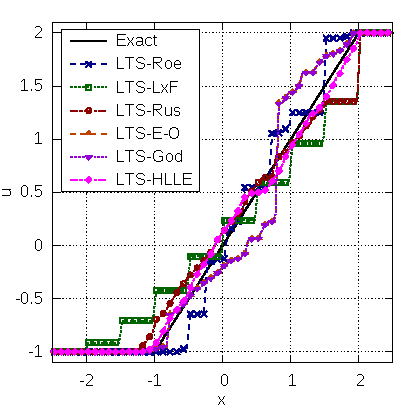
\includegraphics[width=0.48\textwidth]
	{Figures/Scalar/EV-R2-nj100.pdf}}	
	\hspace{0.005\textwidth}
	\subfloat[1000 cells, $ \Delta t = 0.0125 $, 80 time steps]
	{\label{fig:EV-R2-j1000}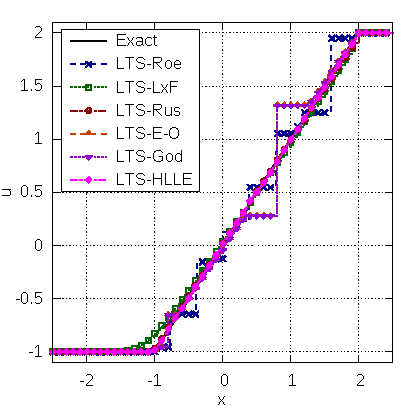
\includegraphics[width=0.48\textwidth]
	{Figures/Scalar/EV-R2-nj1000.pdf}}
	
	\captionsetup{justification=centering}
	
	\caption{Comparison of different LTS methods at $ \bar{C}=5 $ for the Riemann problem \eqref{eq:RP-R2}}
	\label{fig:R2}

\end{figure} 

We can see that the conjectures from \Cref{tabl:EntropyStability} are in agreement with the numerical experiments. A number of numerical experiments for the LTS-HLLE scheme applied to systems of equations implies the same. We refer to Nygaard~\cite{nyg17} for the shallow water equations, and to our papers~\cite{cp2,jp2,jp3} for the Euler equations.
